\chapter{Scheduled Pedestrians and Shared Resources}\label{chap:problem}

\section{Introduction}\label{sec:problem-intro}

This chapter states what we want to build and what makes it hard. \Cref{sec:problem-statement} describes the behavior we want the people of a simulated place to show, gives a one-page overview of how we produce that behavior (\cref{sub:problem-overview}) and lists the functional requirements R1 to R7 that follow from it (\cref{sec:problem-requirements}). \Cref{sec:problem-challenges} then discusses the issues that make these requirements hard to meet in a game engine, which in turn guide the design in \cref{chap:contribution} and the assessment in \cref{chap:conclusions}.

\section{Behavior}\label{sec:problem-statement}

We begin with a population of people in the game engine whose movement follows the boids rules, so that they are capable of following a path and of reacting to their neighbors but have no reason to go anywhere. A scenario has four components: the \emph{environment} $E$, the \emph{population} $A$, the \emph{schedule} $S$ and the \emph{configuration} $C$. The environment holds the walking surfaces, walls, gates, exits and resources, such as desks, counters and tables, each with its own number of places, the schedule is a set of rules, and the configuration sets the clock speed and the optional behaviors. A rule is of the form $r = (a_r, t_r, \alpha_r, g_r)$, where $a_r$ is the person or group of people that the rule applies to, $t_r$ is the authored time of day, $\alpha_r$ is the action and $g_r$ is the target. The rule becomes \emph{eligible} at $e_r = t_r + o_{a}$, where $o_{a} \geq 0$ is an optional per-person offset. The simulation decides when the rule is \emph{dispatched}, at $d_r \geq e_r$, and when the activity \emph{starts}, at $s_r = d_r + q_r + w_r + p_r$, where $q_r$ is the time spent waiting for a free place, $w_r$ the time spent walking and $p_r$ the short positioning at the place before the service starts. The \emph{lateness} of the rule is then $\ell_r = d_r - e_r$, as \cref{fig:problem-timeline} shows.

\begin{figure}[H]
\centering
\begin{tikzpicture}[font=\footnotesize,>=Latex,
  tmark/.style={densely dashed,black!60}]
\draw[->,thick] (0,0) -- (14.6,0) node[below left=2pt and 0pt]{simulated time};
\fill[cPurple!25,draw=cPurple!80!black] (0.2,0.35) rectangle (3.6,0.95);
\node at (1.9,0.65) {previous activity};
\fill[cVerm!25,draw=cVerm!80!black] (3.6,0.35) rectangle (6.4,0.95);
\node at (5.0,0.65) {queued for a place};
\fill[cBlue!25,draw=cBlue!80!black] (6.4,0.35) rectangle (9.4,0.95);
\node at (7.9,0.65) {walk to the station};
\fill[cGreen!30,draw=cGreen!80!black] (9.4,0.35) rectangle (13.4,0.95);
\node at (11.4,0.65) {service (authored duration)};
\draw[tmark] (1.6,-0.15) -- (1.6,1.5) node[above]{$e_r$};
\draw[tmark] (3.6,-0.15) -- (3.6,1.5) node[above]{$d_r$};
\draw[tmark] (6.4,-0.15) -- (6.4,1.5) node[above]{reserved};
\draw[tmark] (9.4,-0.15) -- (9.4,1.5) node[above]{$s_r$};
\draw[tmark] (13.4,-0.15) -- (13.4,1.5) node[above]{released};
\draw[|<->|] (1.6,-0.55) -- node[below]{$\ell_r$} (3.6,-0.55);
\draw[|<->|] (1.6,-1.15) -- node[below]{$s_r - e_r = \ell_r + q_r + w_r + p_r$} (9.4,-1.15);
\end{tikzpicture}
\caption[Timeline of one rule that uses a shared resource]{Timeline of one rule that uses a shared resource, where the short positioning $p_r$ is too small to draw (schematic, not measured data).}
\label{fig:problem-timeline}
\end{figure}

\emph{Given $E$, $A$, $S$ and $C$, the system has to turn the rules into movement and activity such that $\ell_r$, $q_r$ and $w_r$ emerge from the people's schedules, their walking, the capacity of the resources and the layout, rather than being explicitly set by the user. It has to do this with one implementation of a person for all scenarios and have sufficient information for the user to see why an activity started when it did.} A rule is therefore a request that the simulation may defer, and changing the scenario must mean changing $E$, $S$ or $C$, with the person remaining the same.

\subsection{Overview of the approach}\label{sub:problem-overview}

Our approach treats every person in the simulation as someone with a timetable rather than as a particle in a flock. For each person or group of people, a user writes a list of activities, each with the time of day from which it may start and the place where it happens, such as a desk in an office from 08:40 for fifteen minutes or a table in a food court at lunchtime. Nothing in this list says how the person gets there or what happens when the place is taken, because those answers come from the rest of the simulation, whose parts and the signals between them are shown in \cref{fig:architecture}.

When an activity becomes due and the person is free, the person picks a route to the place and walks it, spreading out from the people around them without being pulled off the route by the crowd. Every shared place, such as a desk, a counter, a table or an exit, has a limited number of places, a first-come queue and a service time. A person asks for a place as soon as the activity starts and either receives one at once or joins the queue. Once the place is theirs, the person walks to it, stays for the service time and then frees it, which lets the next person in the queue take the place and lets the person move on to the next step of the activity or to the next item of the timetable. A person who is still busy with something else, such as walking, queueing or being served, keeps the next item waiting until they are free, while an item that has become far too late is dropped.

\begin{figure}[H]
\centering
\begin{adjustbox}{max width=0.8\textwidth}
\begin{tikzpicture}[font=\footnotesize,>=Latex,
  every node/.append style={execute at begin node={\hyphenpenalty=10000\relax}},
  box/.style={draw,rounded corners=2pt,align=center,text width=2.7cm,minimum height=2.0cm,inner sep=3pt},
  wide/.style={draw,rounded corners=2pt,align=center,inner sep=3pt,minimum height=.9cm},
  lab/.style={font=\scriptsize,fill=white,inner sep=1pt,align=center},
  arr/.style={->,thick},
  fb/.style={->,thick,dashed}]
\node[box,fill=cPurple!15,draw=cPurple!80!black] (sched) at (0,0) {{\bfseries Timetable}\\[2pt]Activities of each person: what, where and from when, checked every simulated minute.};
\node[box,fill=cOrange!15,draw=cOrange!80!black] (person) at (3.8,0) {{\bfseries Person}\\[2pt]Does one activity at a time, and a busy person keeps the next one waiting.};
\node[box,fill=cBlue!15,draw=cBlue!80!black] (move) at (7.6,0) {{\bfseries Walking}\\[2pt]Follows a route to the place and is nudged by the people nearby.};
\node[box,fill=cVerm!15,draw=cVerm!80!black] (station) at (11.4,0) {{\bfseries Shared place}\\[2pt]Limited places, a first-come queue and a service time.};
\draw[arr] (sched) -- node[lab,above=3pt]{due\\activity} (person);
\draw[arr] (person) -- node[lab,above=3pt]{destination} (move);
\draw[arr] (move) -- node[lab,above=3pt]{arrival} (station);
\draw[arr] ($(person.north east)+(-.35,0)$) .. controls +(0,.8) and +(0,.8) .. node[lab,pos=.5]{ask for a place: given at once, or queued} ($(station.north west)+(.35,0)$);
\draw[fb] ($(station.north east)+(-.35,0)$) .. controls +(0,1.9) and +(0,1.9) .. node[lab,pos=.5]{done: free the place, start the next step or let the person continue} ($(person.north west)+(.35,0)$);
\node[wide,text width=6.6cm,fill=cGreen!15,draw=cGreen!80!black] (env) at (9.5,-2.95) {{\bfseries Surroundings}\\Walkways, walls, gates, exits, safe areas and where the shared places are};
\node[wide,text width=6.0cm,fill=black!5] (cfg) at (1.9,-2.95) {{\bfseries Scenario setup}\\Which timetable, where people start and which options are on};
\draw[arr] (env.north -| move) -- (move.south);
\draw[arr] (env.north -| station) -- (station.south);
\draw[arr] (cfg.north -| sched) -- (sched.south);
\draw[arr] (cfg.north -| person) -- (person.south);
\node[wide,text width=13.6cm,minimum height=.7cm,fill=cSky!15,draw=cSky!80!black] (obs) at (5.7,-4.65) {{\bfseries Recorder}: notes every request, wait, walk and service of every person};
\draw[fb] (obs.north -| env.south) ++(0,0) -- (env.south);
\end{tikzpicture}
\end{adjustbox}
\caption[Overview of the approach]{Overview of the approach, where the dashed arrow at the top is the signal that lets a person continue once an activity is done.}
\label{fig:architecture}
\end{figure}

The surroundings shape all of this without appearing in the timetable, as walkways set the preferred routes, walls and closed gates block them, exits and safe areas take over when an alarm sounds, and the number and position of the shared places decide where queues form. A separate setup for each scenario only says which timetable to use and where people start. A recorder notes every request, wait, walk and service, so that the gap between the written time of an activity and the time it really started can be explained afterwards. The written time is therefore a request rather than an order, and the actual start depends on what the person is still doing, how far they have to walk and whether the place is free, which is exactly the gap that the evaluation in \cref{chap:applications} measures.

\subsection{Functional requirements}\label{sec:problem-requirements}

\Cref{tab:requirements} lists the functional requirements that this behavior implies. None of them ask for realistic behavior, collision-free motion or the ability to predict a real facility.

\section{Issues}\label{sec:problem-challenges}

\subsection{Purpose versus motion}\label{sub:challenge-purpose}

Boids react to the neighbors in their field of view \citep{reynolds1987flocks}, while purpose is global, individual, and changes throughout the day. If goal forces are added to the steering sum, the flock can pull people away from their goals through weights that mean nothing to the user, and hard-coded purpose turns every activity into a separate piece of code. With the separation of action selection and steering \citep{reynolds1999steering}, purpose should be in the form of readable rules external to the person (using a small vocabulary, \textbf{R1}). Reaching a target around walls and roads requires a path over a navigation mesh \citep{snook2000simplified,mononen2009recast}, but a person who only follows a path loses all the local interactions of the boids. The path will dictate where the person goes, and the boids will dictate how they get through others, while the environment will define which surfaces are preferred and which routes are available (\textbf{R5}).

\begin{table}[H]
\centering
\small
\renewcommand{\arraystretch}{1.1}
\begin{tabular}{|L{0.05\textwidth}|L{0.22\textwidth}|L{0.66\textwidth}|}
\hline
\rowcolor{headgray}\textbf{ID} & \textbf{Name} & \textbf{Requirement} \\
\hline
R1 & Purpose as authored data & Which people do what, when and where is stated in readable files, such as XML schedules, apart from the simulation code, with a small fixed set of actions, and changing activities needs no recompilation. \\ \hline
R2 & Timing under contention & An authored time is the earliest start. Eligible, deferred, dispatched, used-up and dropped rules are defined, no authored minute is skipped, realized times result from the simulation, and durations keep their meaning in every run mode. \\ \hline
R3 & Shared capacity-limited resources & Resources have places, a waiting discipline and a service time, people reserve or queue, places are released on completion or interruption, and multi-stage activities advance on completion. \\ \hline
R4 & Reuse across scenarios & One implementation of a person, one movement layer and one resource model serve different maps and activity patterns, and scenario-specific code is small, isolated and identifiable. \\ \hline
R5 & Environmental constraints & Surfaces, walls, gates, exits and the number of resources shape movement and timing without being restated in rules, and people follow paths while boids shape local motion. \\ \hline
R6 & Observability and measurement & Runs record authored, eligible and realized times, resource events, frame timings and the state of every person in files analysable outside the engine, with documented measures. \\ \hline
R7 & Interactive performance & Scenarios run at 30 frames per second with their authored populations, a faster non-visual mode exists, and cost is measurable as the population grows. \\ \hline
\end{tabular}
\caption[Functional requirements]{Functional requirements that follow from the behavior we want.}
\label{tab:requirements}
\end{table}

\subsection{Timing under contention}\label{sub:challenge-timing}

At 08:40, a person could still be walking from home or could still be waiting, as someone else has the desk. Executing the rule anyway would break the routine, executing the rules strictly in order could delay the shift for the whole day, and waiting indefinitely would let the morning rules run in the afternoon. The system has to define when a rule is eligible, when it is deferred, when it is used up, and when it is dropped. No authored minute may be skipped, even when one frame covers several simulated minutes, and the durations must have the same meaning in every run mode (\textbf{R2}).

\subsection{Shared resources and queues}\label{sub:challenge-resources}

\begin{wrapfigure}{r}{0.5\textwidth}
\centering
\vspace{-0.6\baselineskip}
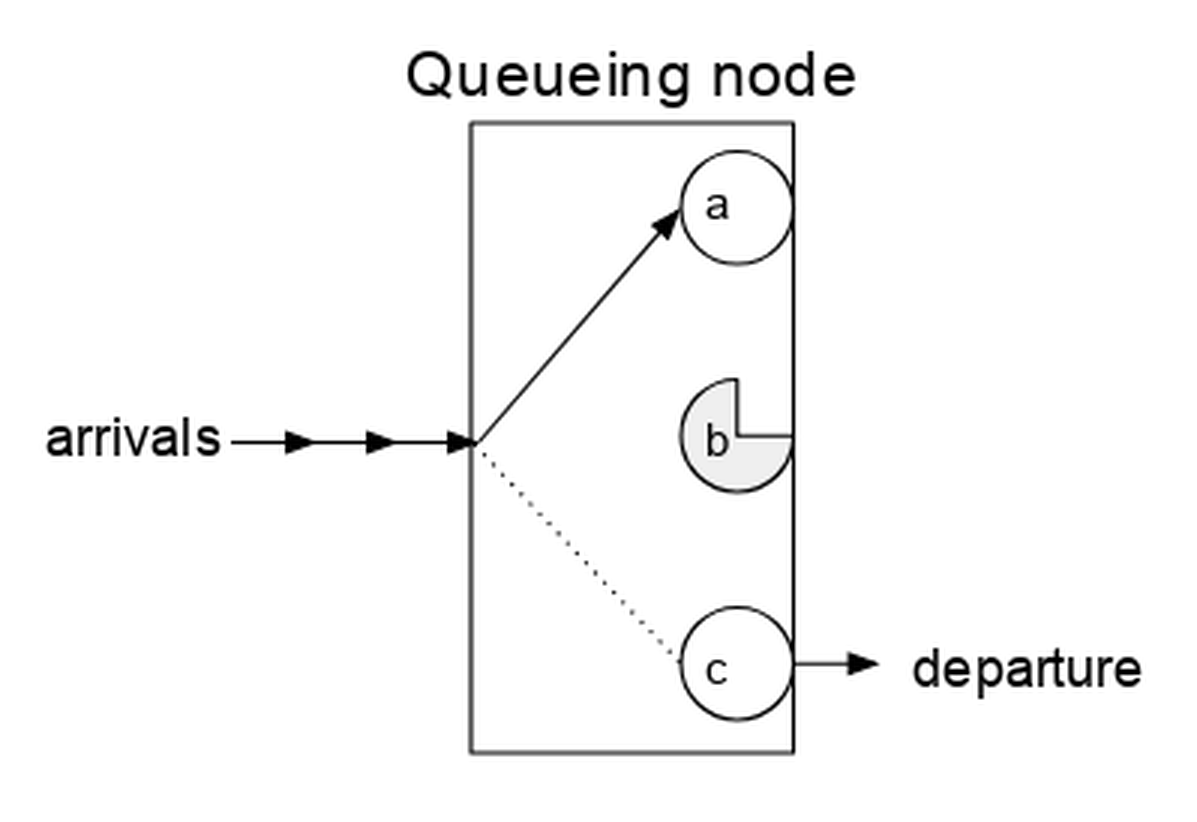
\includegraphics[width=0.48\textwidth]{images/web/queueing_node_x3.png}
\caption[A queueing node]{A queueing node, where arrivals wait for one of several servers and leave after their service (diagram by Dt-rush-8, \href{https://creativecommons.org/licenses/by-sa/4.0/}{CC~BY-SA~4.0}, via \href{https://commons.wikimedia.org/}{Wikimedia Commons}).}
\label{fig:problem-queue}
\vspace{-0.6\baselineskip}
\end{wrapfigure}
Desks, counters, tables and exits are all servers with a capacity, an arrival process, driven here by schedules and walking, and a service time \citep{kendall1953stochastic} (\cref{fig:problem-queue}). The design must decide whether a place is booked on request or on arrival, where the person queues and for which station, and what releases the place. It must also handle a two-stage activity, such as ordering and then eating, so that a person does not hold a table while still queueing at the counter. Smart objects hold the information needed to use them \citep{kallmann1999modeling}, and Unreal Engine's Smart Objects let people claim a slot \citep{epicgames2026smartobjects}. We also need capacity, a queue and a timed service linked to the schedule, with a lifecycle detailed enough to measure the time spent waiting (\textbf{R3}).


\subsection{Reuse across scenarios}\label{sub:challenge-reuse}

The same implementation of a person, movement layer and resource model should serve a daily urban routine, a shopping center, an evacuation and a directed-flow test, with the variations expressed in schedules, maps and configuration. Full reuse is difficult, because an evacuation needs exit choice and a routine needs a home, so scenario-specific code should be small and identifiable (\textbf{R4}), and the environment should absorb variations such as an extra table or a gate opened by a button (\textbf{R5}).

\subsection{Measurement and performance}\label{sub:challenge-measurement}\label{sub:challenge-performance}

A person who stands still could be queued, deferred, blocked or stuck, so watching a run does not reveal their state. The system must therefore record rule times, station events, trips and frame times, document what each measure means and reproduce the analysis from the files (\textbf{R6}). It also shares each 33~ms frame with rendering and animation, and naive boids compare every pair of people (\cref{sub:complexity}), so the scenarios must run interactively at a cost that can be measured (\textbf{R7}).
